\documentclass[11pt, a4paper]{article}

\usepackage{hyperref}
\usepackage{graphicx}

\begin{document}

\title{Supplementary Information for ``VPsearch: a package for fast exact
  sequence similarity search''}
\date{}

\maketitle
\tableofcontents

\section{Algorithmic description}

In this section we describe particular implementation choices that were made
during the design of VPsearch. For a general description of how the vantage
point algorithm works, we refer to the original literature
(\cite{1991-uhlmann-SatisfyingGeneralProximity},
\cite{1993-yianilos-DataStructuresAlgorithms}).

\subsection{Choice of distance function}

Vantage point trees require the selection of a distance function between
elements of the space to be indexed. For nucleotide sequences, a distance
function $S(q, r)$ between two sequences $q$ and $r$ can be defined by means of
the Needleman-Wunsch sequence alignment algorithm, and is given by
\begin{equation} \label{eq:similarity}
   S(q, r) = NW(q, q) + NW(r, r) - 2NW(q, r),
\end{equation}
where $NQ(q, r)$ is the Needleman-Wunsch alignment distance between two
sequences $q$ and $r$ using the nuc44 substitution matrix.


\subsection{Choice of the vantage point}

In the original description of the concept of vantage point trees, the vantage
point is chosen at random during the construction of each level of the tree. In
our construction the vantage point is chosen semi-deterministically so that the
vantage point is maximally capable of separating the remaining sequences. To
achieve this, 5 candidate vantage point sequences are sampled at random,
together with 20 ``test'' sequences. For each candidate vantage point, the
distance to all test sequences is computed using the distance function defined
in (\ref{eq:similarity}). The retained vantage point is then the one that
maximizes the variance in the distance to the test sequences.

\section{Preparation of the sequence database}

We downloaded version 138 of the Silva reference database from
\url{https://zenodo.org/record/4587955}. The v4 region was excised using
ProbeMatch, part of the RDPTools suite, with the standard 515f/806r
primers. Sequences were rejected if there were more than 3 mismatches in the
location of the forward or reverse primer, or if the length of the v4 region
was less than 250 or more than 300 base pairs. This step resulted in 42940 of
the original 452064 sequences (9.50\%) being rejected.

The v4 sequences were then deduplicated, resulting in a database consisting of
230013 unique v4 sequences with taxonomic information. As ggsearch36 is not
able to handle sequence IDs longer than 120 characters, the sequence IDs were
recoded and the original sequences IDs were stored for use in downstream
analysis.

The deduplicated database of 230013 sequences was the starting point for the
comparison between the different similarity search tools. For the comparison of
lookup time as a function of database size, we took random samples of the full
database of 100, 1000, 10000, and 100000 sequences.

The processed databases, as well as scripts to deterministically regenerate
them, can be found from the GitHub page accompanying this paper, at
\url{https://github.com/jvkersch/vpsearch-paper}.

\section{Comparison with NMSLIB}

We compared our implementation of the vantage-point search algorithm with the
implementation provided by the NMSLIB package
(\cite{2013-boytsov-EngineeringEfficientEffective}) available from
\url{https://github.com/nmslib/nmslib}. To this end, we modified NMSLIB to
calculate the Needleman-Wunsch distance using Parasail (code available from our
custom fork of NMSLIB at
\url{https://github.com/jvkersch/nmslib/tree/space-nw}). We find that NMSLIB is
comparable in runtime performance to our native implementation, both as far as
lookup time is concerned (see Fig.~\ref{fig:timing}) and for taxonomic
accuracy. However, there are two drawbacks in the code which currently preclude
the use of NMSLIB for our application:

\begin{itemize}
\item NMSLIB currently provides no way of saving a persistent vantage-point
  search tree to disk, so that the tree has to be rebuilt with every new query
  invocation.
\item NMSLIB is not natively aware of biologically inspired distance functions,
  and needs to be modified before it can use e.g. the Needleman-Wunsch
  distance.
\end{itemize}

\begin{figure} \label{fig:timing}
  \centering
  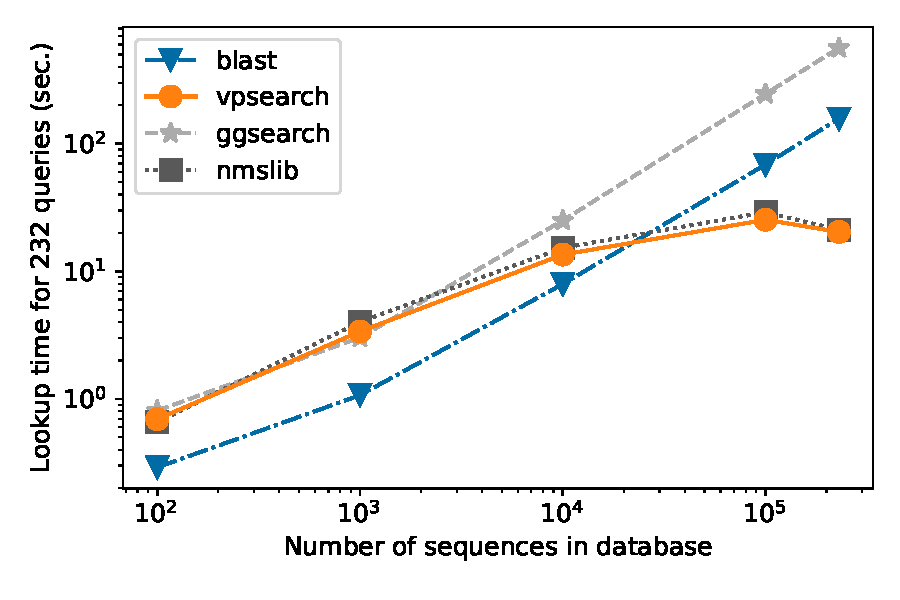
\includegraphics[scale=0.5]{execution-time-nmslib.pdf}
  \caption{Sequence lookup time for 232 sequences as a function of the size of
    the database. This figure includes timings obtained with our custom build
    of NMSLIB and shows that lookup times between NMSLIB and our vantage-point
    tree implementation are roughly comparable.}
\end{figure}

\bibliographystyle{unsrt}
\bibliography{vpsearch-paper}

\end{document}
